%
% File acl2012.tex
%
% Contact: Maggie Li (cswjli@comp.polyu.edu.hk), Michael White (mwhite@ling.osu.edu)
%%
%% Based on the style files for ACL2008 by Joakim Nivre and Noah Smith
%% and that of ACL2010 by Jing-Shin Chang and Philipp Koehn


\documentclass[11pt]{article}
\usepackage{acl2012}
\usepackage{times}
\usepackage{latexsym}
\usepackage{amsmath}
\usepackage{multirow}
\usepackage{url} 

\usepackage{float}
\usepackage{lingmacros}
\usepackage{tree-dvips}
\usepackage{graphicx}
\usepackage{supertabular}
\usepackage{array}
\usepackage[english]{babel}



\DeclareMathOperator*{\argmax}{arg\,max}
\setlength\titlebox{6.5cm}    % Expanding the titlebox

\title{Predicting Viewer Reactions of Debate Performances}

\author{Peter Enns \\
  Linguistics Department \\
  University of Maryland \\
  {\tt slunk@terpmail.umd.edu} \\\And
  Isaac Julien \\
  Computer Science Department \\
  University of Maryland \\
  {\tt ijulien6@gmail.com} \\ \\\And
  Alex Memory \\
  Computer Science Department \\
  University of Maryland \\
  {\tt memory@cs.umd.edu} \\
  }

\date{}

\begin{document}
\maketitle
\begin{abstract}
  There is growing interest in the factors that influence audience reactions to political debate and in predicting over-all reactions to a particular debate performance.  Using a unique live polling data source, we view this as a supervised classification task using the topics discussed by the debaters as the features and the volume and sentiment of reactions as the label to predict.  To evaluate our topic-based approach, we compare to a baseline using n-gram features and we also compare performance from automatically- and manually-coded topics.  Finally, we consider a related task in which we predict reactions of individual audience members.
\end{abstract}

\section{Introduction}
We predict reactions of viewers to debate performances.  We did this and that.


\section{Project Plan}
%!TEX root =  cl2-lda.tex

This project focuses on whether topic-based features can predict a viewer's reaction
to a presidential debate.
Alex implemented and evaluated the baseline classification scheme for predicting
reactions to turns in the debate.
Peter generated topics for the debate corpus using LDA and evaluated classification
performance using these.
Isaac evaluated the performance of hand-chosen topic labels for this task,
and the prediction of individual user reactions.
All were involved in substantial data analysis and project assembly.

\section{Data and Resources}
%!TEX root =  cl2-lda.tex

\subsubsection{Data}

We used the annotated October 3rd 2013 presidential debate and the annonated presidential debate corpus (both obtained through Philip Resnik).
Together, the corpora are approximately 12,000 lines long.
Each line is comprised of a statement and metadata about that statement (speaker, tone, topic, etc...).
We had to preprocess the corpora, first by tokenizing it into turns in each debate, and second by performing normal preprocessing steps (e.g., tokenizing into words and removing stopwords).

In addition to the corpora, we also used the reaction data from ReactLabs (also provided by Philip Resnik).
This dataset contained 193,287 reactions by ReactLabs app \emph{users} to the October 3rd presidential debate.
Each line in the file corresponded to a single reaction (Romney:Disagree, Obama:Spin, etc...) with a timestamp and metadata about the user who submitted the reaction.

The reactions started a half hour before the debate and continued for a half hour after the debate -- we discard reactions from these time periods -- and over all the reactions are tightly clustered in time; see Fig.~\ref{fig:reactionseachturn}

\begin{figure}[]
	\centering
	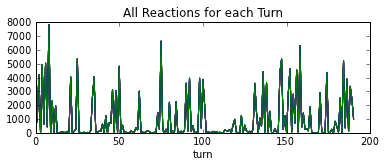
\includegraphics[scale=0.6]{Figures/reactions_for_each_turn.png}
	\caption{Reactions by all users for each turn.}
	\label{fig:reactionseachturn}
\end{figure}

The annotated debate corpus and reactions data set are synchronized allowing us to associate reactions to each \emph{turn} taken by a candidate during the debate.  However, it is common for users to react to someone who is not speaking.  In Fig.~\ref{fig:reacts_while_others_talk} we see that it is especially common for users to react to the moderator while one of the candidates is speaking, perhaps because the moderator speaks for shorter periods of time than the candidates.  Also an even larger number of reactions to the candidates are assigned to one another or the moderator, perhaps because the users are still reacting to a candidate's last turn.

\begin{figure}[]
	\centering
	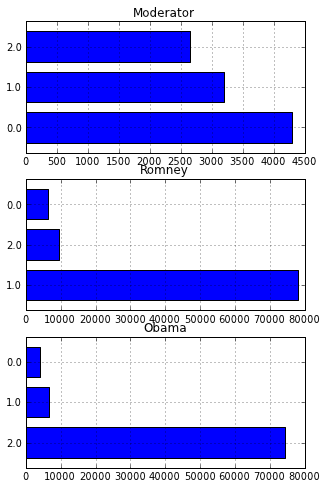
\includegraphics[scale=0.5]{Figures/reactions_while_others_are_talking}
	\caption{Reactions to the moderator (top), Romney (middle) or Obama (bottom) while speaker 0 (Moderator), 1 (Romney) or 2 (Obama) was talking.}
	\label{fig:reacts_while_others_talk}
\end{figure}

For this reason, we limit the reactions we consider to those where the reaction is associated with the person \emph{currently speaking}.  This reduces the 	number of reactions records by approximately 21\%.

Over all, we see in Fig.~\ref{fig:kinds_of_reactions_to_speakers} that reactions to Obama are overwhelmingly agreement, while a high percentage of reactions to Romney are dodge, spin or disagree reactions.

\begin{figure}[]
	\centering
	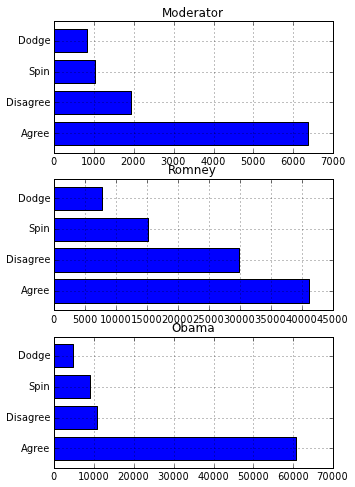
\includegraphics[scale=0.5]{Figures/kinds_of_reactions_to_speakers}
	\caption{Frequencies of reactions of each type over the course of the debate for the moderator (top), Romney (middle) and Obama (bottom).}
	\label{fig:kinds_of_reactions_to_speakers}
\end{figure}

However, this is not surprising, given the stated preferences of the users at the beginning of the debate, cf. Fig.~\ref{fig:preferred_candidates}; the users prefer Obama over Romney by over two to one.  We will see that this imbalance may create issues of bias in training examples once we begin to predict reactions of Obama or Romney supporters for what is being said in each turn.

\begin{figure}[]
	\centering
	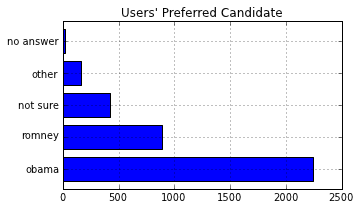
\includegraphics[scale=0.5]{Figures/preferred_candidates}
	\caption{Frequencies of each candidate as preferred by the users reacting to the debate.}
	\label{fig:preferred_candidates}
\end{figure}


\subsubsection{Resources}

We use the Machine Learning for Language Toolkit (Mallet) for several tasks in the project.
First, we use it to infer topics from the debate corpus.
Second, we use it to train several different classifiers (Decision Tree, MaxEnt, Naive Bayes).

We also use several Python modules for various jobs.
We use the natural language toolkit (NLTK) for preprocessing tasks (e.g., sentence and word tokenization, removing stopwords, etc...).
We use NumPy, SciPy, matplotlib, and Pandas for data analysis.
Finally, we use sqlite3 to store the reactions data in a format that is easier to filter.


\section{The Problem}
%!TEX root =  cl2-lda.tex

The high level description of what we decided to do with the data and why.

\subsection{High Level Task}

\subsection{Expected Outcomes}



\section{Models and Algorithms}
%!TEX root =  cl2-lda.tex

For the task of predicting user reactions given features generated from the debate text, we use different algorithms for feature generation and for prediction.  To generate topic features from text, we use LDA~\cite{blei_latent_2003} as implemented by~\cite{mccallum_mallet:_2002}.  To predict the user reactions we use decision tree, maximum entropy and naive Bayes classifiers as implemented in~\cite{mccallum_mallet:_2002} or~\cite{bird_nltk:_2006}.

We parameterize each algorithm for each of our tasks and describe how we choose the particular the parameter settings in Section~\ref{sec:evaluation}.

\section{Evaluation}
\label{sec:evaluation}
%!TEX root =  cl2-lda.tex

\subsection{Predicting Reactions with LDA Topics}
%!TEX root =  cl2-lda.tex

Latent Dirichlet Allocation (LDA) is a hierarchical Bayesian model.
In LDA, documents are modeled as random mixtures over latent topics and topics are distributions over words.

We ran Mallet's implementation of LDA on our training data (the October 3rd presidential debate and the presidential debate corpus) with hyperparameter optimization on.
The data was split into debate turns and stopwords were removed.
Figure \ref{fig:ldatopics} shows the top terms for each topic distribution generated by one run of LDA.
We chose to model 19 topics in order to agree the number of topics in Boydstun's annotations.
The features for each document in our predictive models were the proportions of topics LDA allocated to those documents.

Surprisingly, using LDA topic proportions actually performed \textit{better} for task 1 and task 2 with the Decision Tree and Maximum Entropy classifiers (Tables \ref{tab:task1lda} and \ref{tab:task2lda}).
Possibly even more perplexingly, the Naive Bayes classifier performed abyssmally at all three tasks with these features.
Although it was more than adequate for task 1 and task 2, it fell short of the coded topic classifiers for task three (Table \ref{tab:task3lda}).


\begin{figure*}
\begin{flushleft}
\tablefirsthead{}
\tablehead{}
\tabletail{}
\tablelasttail{}
\begin{supertabular}{|m{4.8087597in}|m{1.1906599in}|}
\hline
{\selectlanguage{english} Top Terms} &
{\selectlanguage{english} Topic}\\\hline
{\selectlanguage{english} president america country states united didn made today respect \ difference american don fact
mistake make policy decisions question kids decision} &
{\selectlanguage{english} Incoherent}\\\hline
{\selectlanguage{english} campaign people country foreign american fact issues town lobbyists house congress tough white
honor running campaigns interested pledge john character} &
{\selectlanguage{english} Campaigning (?)}\\\hline
{\selectlanguage{english} \textbf{health care plan insurance medicare costs }cost government give companies
\textbf{system} buy seniors choice program lower billion \textbf{private} provide \textbf{premiums}} &
{\selectlanguage{english} Healthcare}\\\hline
{\selectlanguage{english} \textbf{drugs} don act \textbf{law} congress rights bill \textbf{crime} line \textbf{drug}
\textbf{police} \textbf{protect} patriot border \textbf{enforcement} legislation citizens fact enterprise
\textbf{fighting}} &
{\selectlanguage{english} Law Enforcement}\\\hline
{\selectlanguage{english} ve people don make ll time back work things years put lot good country america important
american president point thing} &
{\selectlanguage{english} Incoherent}\\\hline
{\selectlanguage{english} \textbf{iraq} \textbf{afghanistan} senator \textbf{troops} \textbf{strategy} obama
\textbf{pakistan} \textbf{russia} \textbf{war} \textbf{georgia} \textbf{qaeda} \textbf{al} mccain \textbf{military}
situation states understand russians \textbf{defeat} united} &
{\selectlanguage{english} Foreign Conflict}\\\hline
{\selectlanguage{english} \textbf{jobs} \textbf{trade} free agreement \textbf{job} country fair \textbf{industries}
\textbf{workers} \textbf{overseas} \textbf{business} standards base defense agreements wage century \textbf{pay}
minimum growing} &
{\selectlanguage{english} Jobs}\\\hline
{\selectlanguage{english} \textbf{governor} \textbf{romney} government \textbf{federal} \textbf{states} board approach
\textbf{obamacare} repeal conditions fact reason replace difference \textbf{cost} military investments crisis
opportunity \textbf{Massachusetts}} &
{\selectlanguage{english} Health Insurance Reform (?)}\\\hline
{\selectlanguage{english} \textbf{world} \textbf{war} \textbf{military} \textbf{troops} \textbf{national}
\textbf{security} \textbf{forces} \textbf{army} peace russia europe \textbf{nuclear} \textbf{draft} general question
\textbf{defense} \textbf{cold} union superpower democracy} &
{\selectlanguage{english} Defense}\\\hline
{\selectlanguage{english} \textbf{nuclear} \textbf{iran} \textbf{north} \textbf{korea} president \textbf{weapons}
\textbf{talks} threat senator united mccain \textbf{proliferation} sanctions countries israel involved china table
\ \ \ \ states ambassador} &
{\selectlanguage{english} Nuclear Weapons}\\\hline
{\selectlanguage{english} \textbf{education} \textbf{school} \textbf{schools} \textbf{child} money \textbf{children}
\textbf{kids} america system job \textbf{teachers} state \textbf{public} abortion program funding college continue
choice \ \ aids} &
{\selectlanguage{english} Education}\\\hline
{\selectlanguage{english} mr president \textbf{question} \textbf{senator} \textbf{minute} perot bush governor kerry
\textbf{minutes} clinton seconds \textbf{answer} \textbf{audience} \textbf{tonight} \textbf{debate} \textbf{questions}
presidential \ candidates sir} &
{\selectlanguage{english} Debate Phrases}\\\hline
{\selectlanguage{english} senator obama voted spending senate states united record party opposed constitution fought
reform bill marriage friends times issue justice \ completely} &
{\selectlanguage{english} Legislative Branch (?)}\\\hline
{\selectlanguage{english} \textbf{iraq} \textbf{war} world \textbf{saddam} \textbf{hussein} plan troops \textbf{weapons}
free opponent \ \ \ \ \textbf{bin} \textbf{osama} \textbf{laden} \textbf{terror} win wrong safe threat strong
intelligence} &
{\selectlanguage{english} Middle East / Terrorism}\\\hline
{\selectlanguage{english} \textbf{energy} \textbf{oil} \textbf{nuclear} \textbf{fuel} percent \textbf{technology}
\textbf{power} reduce stem united companies \textbf{coal} \textbf{drilling} \textbf{clean} \textbf{wind} states
\textbf{solar} \textbf{science} mccain issue} &
{\selectlanguage{english} Energy}\\\hline
{\selectlanguage{english} congress people economic years mr government american governor economy clinton control growth
spend social program change country interest programs jobs} &
{\selectlanguage{english} Clinton Years Economy (?)}\\\hline
{\selectlanguage{english} \textbf{tax} \textbf{taxes} \textbf{cut} \textbf{jobs} billion spending people \textbf{middle}
small \textbf{percent} \ \ \ \ plan pay \textbf{class} america \textbf{raise} budget \textbf{business} money
\textbf{income} deficit} &
{\selectlanguage{english} Taxes}\\\hline
{\selectlanguage{english} mccain sen senator obama crisis \textbf{economy} \textbf{street} \textbf{financial} question
\textbf{banks} \textbf{wall} \textbf{policy} regulation \textbf{economic} homes americans tonight system package fix} &
{\selectlanguage{english} Economy (?)}\\\hline
{\selectlanguage{english} \textbf{children} \textbf{people} \textbf{women} \textbf{family} person \textbf{love} american
\textbf{faith} \textbf{dream} \textbf{life} \textbf{values} great \textbf{woman} strong part \textbf{laughter}
\textbf{god} \textbf{personal} \textbf{wife} \textbf{daughters}} &
{\selectlanguage{english} Pathos}\\\hline
\end{supertabular}
\end{flushleft}
\caption{LDA topics}
\label{fig:ldatopics}
\end{figure*}

\begin{table}[H]
\begin{centering}
\begin{tabular}{ l | l | l }
Classifier & Obama voters & Romney voters \\
\hline
DecTree & \textbf{0.71} (0.05) &  \textbf{0.71} (0.07) \\
MaxEnt & \textbf{0.70} (.06) &  \textbf{.68} (.05) \\
Naive & \textbf{0.20} (.05) &  \textbf{.68} (.04) \\
\end{tabular}
\caption{Task 1 (lda features): Accuracy and StdDev}
\label{tab:task1lda}
\end{centering}
\end{table}

\begin{table}[H]
\begin{centering}
\begin{tabular}{ l | l | l }
Classifier & Obama Voters & Romney Voters \\
\hline
DecTree & \textbf{0.76} (0.08) &  \textbf{0.70} (.06) \\
MaxEnt & \textbf{0.74} (0.05) &  \textbf{0.71} (0.09) \\
Naive & \textbf{0.23} (0.04) &  \textbf{0.21} (0.05) \\
\end{tabular}
\caption{Task 2 (lda features): Accuracy and StdDev}
\label{tab:task2lda}
\end{centering}
\end{table}

\begin{table}[H]
\begin{centering}
\begin{tabular}{ l | l | l }
Classifier & Obama Voters & Romney Voters \\
\hline
DecTree & \textbf{0.74} (0.07) &  \textbf{0.77} (0.05) \\
MaxEnt & \textbf{0.70} (0.10) &  \textbf{0.71} (0.07) \\
Naive & \textbf{0.22} (0.05) &  \textbf{0.26} (0.04) \\
\end{tabular}
\caption{Task 3 (lda features): Accuracy and StdDev}
\label{tab:task3lda}
\end{centering}
\end{table}




\subsection{Predicting Reactions with Labeled Topics}

[Boydstun et. al, 2013] labels each phrase in the October 4th, 2012 debate corpus with a topic ID. Each ID corresponds to a significant topic in the debate, such as "Defense" or "Labor, Employment, and Immigration." Unlike the topics found by LDA, these are hand-selected, with a single topic per phrase instead of a distribution over topics.

We are interested in whether using these hand-labeled topics, as opposed to the topics discovered using LDA, will improve or worsen performance predicting users' reactions to the debate.

Since we are working at the turn level, not the phrase level, we assimilate all topic IDs within a turn into a distribution over topics for that turn.

As before, each labeled topic present in the corpus is a feature. For a given turn, the value of that feature is the fraction of phrases within the turn labeled with that topic.

Once again we evaluate classification accuracy on three tasks, or labels: Whether a turn generates more or less than the median number of reactions per second, whether a turn generates more 'agree' or 'disagree' reactions, and whether a turn generates more or less than the median number of spin or dodge reactions per second.

Classification is done with Mallet, using Decision Tree, Maximum Entropy, and Naive Bayes classifiers. We perform 10-fold cross-validation using the 197 turns to calculate test accuracy and standard deviation:

\begin{table}[H]
\begin{centering}
\begin{tabular}{ l | l | l }
Classifier & Obama voters & Romney voters \\
\hline
DecTree & \textbf{0.695} (.131) &  \textbf{.719} (.150) \\
MaxEnt & \textbf{0.498} (.146) &  \textbf{.386} (.129) \\
Naive & \textbf{0.454} (.142) &  \textbf{.386} (.130) \\
\end{tabular}
\caption{Task 1 Accuracy and StdDev}
\end{centering}
\end{table}

\begin{table}[H]
\begin{centering}
\begin{tabular}{ l | l | l }
Classifier & Obama voters & Romney voters \\
\hline
DecTree & \textbf{0.519} (.095) &  \textbf{.455} (.090) \\
MaxEnt & \textbf{0.577} (.092) &  \textbf{.562} (.141) \\
Naive & \textbf{0.589} (.093) &  \textbf{.567} (.144) \\
\end{tabular}
\caption{Task 2 Accuracy and StdDev}
\end{centering}
\end{table}

\begin{table}[H]
\begin{centering}
\begin{tabular}{ l | l | l }
Classifier & Obama voters & Romney voters \\
\hline
DecTree & \textbf{0.803} (.106) &  \textbf{.805} (.150) \\
MaxEnt & \textbf{0.823} (.122) &  \textbf{.813} (.154) \\
Naive & \textbf{0.823} (.122) &  \textbf{.813} (.154) \\
\end{tabular}
\caption{Task 3 Accuracy and StdDev}
\label{tab:task3boydstun}
\end{centering}
\end{table}

For each classification task, we also keep track of the features that the Mallet Decision Tree learner selects most frequently for having the highest information gain. We can then look up the corresponding topics for the most valuable features.

\begin{table*}[H]
\begin{centering}
\begin{tabular}{| l | l | l |}
\hline
  & Best feature (Obama) & Best Feature (Romney) \\
\hline
Task 1 & labor/employment/immigration & government operations \\
	    & education & macroeconomics \\
	    & health & education \\
	    \hline
Task 2 & labor/employment/immigration & labor/employment/immigration \\
	    & government operations & education \\
	    & social welfare & macroeconomics  \\
	    \hline
Task 3 & candidate personal information & health \\
	    & social welfare & government operations \\
	    & labor/employment/immigration & candidate personal information \\
	    \hline
\end{tabular}
\caption{3 Features with highest information gain}
\end{centering}
\end{table*}

The Decision Tree classifier performs by far the best on Task 1, with $69.5\%$  accuracy on reactions by Obama supporters and $71.9\%$ accuracy on reactions by Romney supporters. The MaxEnt and Naive Bayes classifiers perform poorly. On Task 2, all classifiers perform surprisingly poorly, with the best accuracy being $58.9\%$ using a Naive Bayes classifier. The best performance is on Task 3, on which all three classifiers score in the low $80\%$ range. The MaxEnt and Naive Bayes classifiers score the highest with $82.3\%$ and $81.3\%$ accuracy on reactions by Obama and Romney supporters, respectively.



\subsection{User Reactions}

In the previous sections, we predict reactions to a turn based on the topics present in the turn. We find that we can do this reasonably well for some types of prediction, and also learn what topics contribute most certain reactions.

We can also ask what topics cause an individual user to react, rather than users in general. The label for prediction then becomes that user's reaction, and the features become the topics present in the discussion at the time of the reaction.

However, since we are now working at the individual level, we can also use features based on a user's responses to the ReactLabs survey questions, which we will call "user features." These include questions such as gender and political party, and also questions that ask the user to indicate agreement with one party or another on specific issues with a value between 0 and 100.

We are primarily interested in 1.) how well we can predict user reactions given user features and topic features, and 2.) how much topic features contribute to classification accuracy. Topic features are determined based on the turn in which the reaction occurs. We use features derived from both LDA topics and the Boydstun labeled topics. Labels are the 12 possible user reactions ("$Obama|Romney|Moderator : Agree|Disagree|Spin|Dodge$"). We use 10,000 reactions for 10-fold cross-validation.

\begin{table*}[H]
\begin{centering}
\begin{tabular}{ l | l | l | l }
Classifier & User features only & User + LDA & User + Boydstun \\
\hline
Decision Tree & \textbf{0.389} (.018) & \textbf{0.397} (.016) &  \textbf{.388} (.014) \\
Maximum Entropy & \textbf{.452} (.019) & \textbf{0.517} (.012) &  \textbf{.508} (.022) \\
Naive Bayes & \textbf{.443} (.020) & \textbf{0.481} (.012) &  \textbf{.460} (.013) \\
\end{tabular}
\caption{User reaction classification: accuracy and standard deviation}
\end{centering}
\end{table*}

We also plot confusion matrices using the best-performing classifier for both user features alone and user features combined with topic features.

\begin{figure}[H]
	\centering
	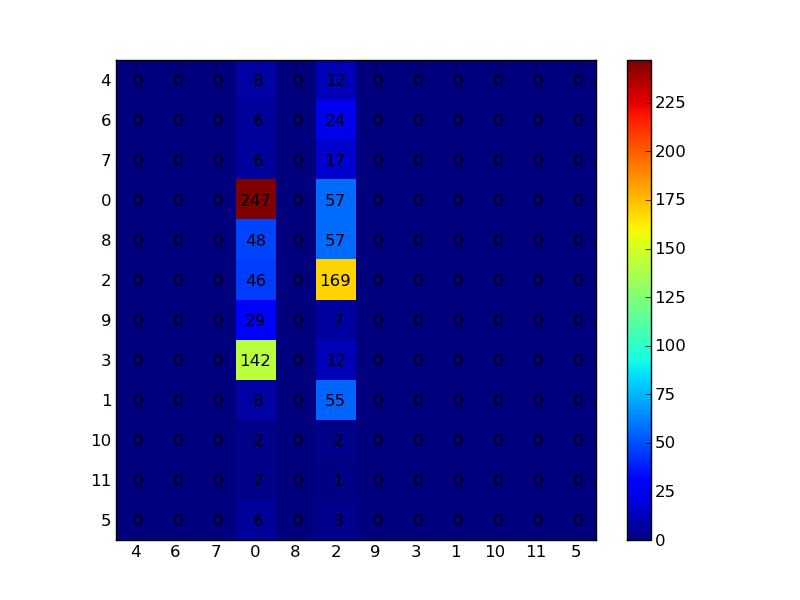
\includegraphics[scale=0.35]{Figures/no_topic_features_confusion.png}
	\caption{Confusion Matrix: Classification with user features only}
	\label{fig:useronlyconfusion}
\end{figure}

\begin{figure}[H]
	\centering
	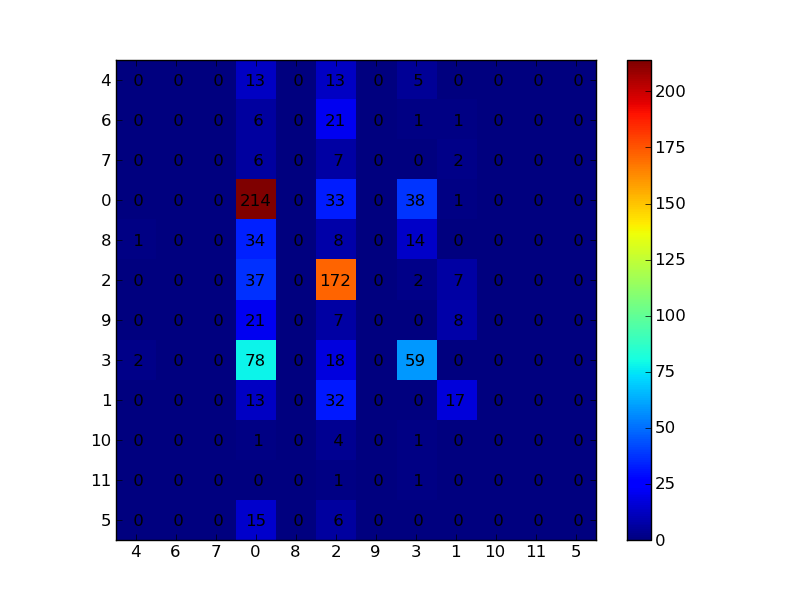
\includegraphics[scale=0.35]{Figures/boydstun_confusion.png}
	\caption{Confusion Matrix: Classification with user and topic features}
	\label{fig:boydstunconfusion}
\end{figure}


\begin{table}[H]
\begin{centering}
\begin{tabular}{ l | l | l | l }
 Code & Topic & Code & Topic \\
\hline
4 & Moderator:Agree & 9 & Romney:Dodge \\
6 & Obama:Spin & 3 & Romney:Disagree \\
7 & Obama:Dodge & 1 & Obama:Disagree \\
0 & Obama:Agree & 10 & Moderator:Spin \\
8 & Romney:Spin & 11 & Moderator:Dodge \\
2 & Romney:Agree & 5 & Moderator:Disagree \\
\end{tabular}
\caption{Topic code key}
\end{centering}
\end{table}

As expected, using topic-based features in addition to user features improves classification accuracy. The maximum entropy classifier shows the greatest improvement, increasing from $45.2\%$ accuracy to $51.7\%$ accuracy.

This is an interesting result, since the maximum entropy classifier is the one classifier that makes no independence assumptions between the features. The increase in accuracy suggests that it does a better job of integrating the user features with the topic features. For instance, the maximum entropy classifier might be more capable of classifying the reaction of a user who indicates a certain topic is more important to him during a turn in which that topic is present.

From the confusion matrices, one can see that the majority of predictions fall into labels 0 and 2, corresponding to "Obama:Agree" and "Romney:Agree." In Figure \ref{fig:useronlyconfusion}, labels for "Romney:Disagree" are often confused with labels for "Obama:Agree." This makes sense, since a user who disagrees with Romney most likely agrees with Obama. Including topic features results in more predictions of labels 3 and 1, "Obama:Disagree" and "Romney:Disagree" (Figure \ref{fig:boydstunconfusion}).

\subsection{Predicting Reactions with N-Grams}
%!TEX root =  cl2-lda.tex

Predicting users' reactions to the debate based on n-grams from the text of the each turn taken by the candidates is a simple approach, and we are interested to see how well the topic-based methods compare to it in terms of performance.

On all the tasks, we predict the responses to turns using Decision Tree, Maximum Entropy and Naive Bayes classifiers; we used the implementations of these classifiers from NLTK\textbf{ref}.  We measure our final accuracy on all tasks with 10-fold cross validation.  

To extract n-gram features from the transcripts of the turns, we began by splitting the text into tokens using the English tokenizer from NLTK.  We then removed punctuation, numbers and stop-words; and then converted all n-grams to lower-case.  Finally, we produced a single feature for each unique n-gram in each turn indicating is presence (not the count of tokens for that n-gram).  

For our evaluation, we considered either unigrams or bigrams as features.  To determine the number of n-gram features to use to avoid overfitting, we varied their number while evaluating mean accuracy during repeated random sub-sampling validation.  To select which n-grams to include among the features, we selected the n-grams with the most frequent unigrams first.

In Table~\ref{tab:task1unigrams} we see that on \textbf{Task 1} the decision tree performed best over all, while on \textbf{Task 2}, naive Bayes performed very well when predicting reactions of Obama voters but not for Romney voters, cf. Table~\ref{tab:task2unigrams}.  Finally, we see in~\ref{tab:task3unigrams} that on \textbf{Task 3}, maximum entropy performed best over all while naive bayes continued to struggle at predicting reactions of Romney voters.

\begin{table}[H]
\begin{centering}
\begin{tabular}{ l | l | l }
Classifier & Obama voters & Romney voters \\
\hline
DecTree & \textbf{0.84} (0.07) &  \textbf{0.83} (0.17) \\
MaxEnt & \textbf{0.78} (.16) &  \textbf{.84} (.16) \\
Naive & \textbf{0.75} (.09) &  \textbf{.77} (.15) \\
\end{tabular}
\caption{Task 1 (unigram features): Accuracy and StdDev}
\label{tab:task1unigrams}
\end{centering}
\end{table}

\begin{table}[H]
\begin{centering}
\begin{tabular}{ l | l | l }
Classifier & Obama voters & Romney voters \\
\hline
DecTree & \textbf{0.74} (0.22) &  \textbf{0.83} (0.12) \\
MaxEnt & \textbf{0.76} (.16) &  \textbf{.80} (.06) \\
Naive & \textbf{0.87} (.12) &  \textbf{.50} (.12) \\
\end{tabular}
\caption{Task 2 (unigram features): Accuracy and StdDev}
\label{tab:task2unigrams}
\end{centering}
\end{table}

\begin{table}[H]
\begin{centering}
\begin{tabular}{ l | l | l }
Classifier & Obama voters & Romney voters \\
\hline
DecTree & \textbf{0.83} (0.14) &  \textbf{0.80} (0.15) \\
MaxEnt & \textbf{0.86} (.09) &  \textbf{.84} (.13) \\
Naive & \textbf{0.81} (.11) &  \textbf{.49} (.23) \\
\end{tabular}
\caption{Task 3 (unigram features): Accuracy and StdDev}
\label{tab:task3unigrams}
\end{centering}
\end{table}



\section{Discussion}
%!TEX root =  cl2-lda.tex

\subsection{Results}

The unigram feature baseline tends to outperform both hand-labeled and LDA topic features. From the experiments we perform, it seems that individual words in the text are better predictors of reaction than topics inferred from the text.

However, using topics for classification does provide some interesting analysis on how users respond to certain topics. In Section 6.2, we learn which hand-labeled topics tend to generate more responses, and see that when a candidate resorts to personal anecdote the audience often interprets it as a "spin" or "dodge."

With the exception of Naive Bayes classifiers, it seems to be the case that simple LDA topics work well enough for predicting reactions to use them instead of coded topics. 
Unfortunately, it seems like the good performance is difficult to interpret and possibly very fragile.
Using vanilla LDA to obtain features for classification is probably not the best choice.

Finally, we see that using topic-based features boosts the performance of predicting individual users' reactions when combined with demographic features.

\subsection{Future Directions}

One direction for future work is to try out more complex topic models.
It would be interesting to see if you get better topics and/or predictions if they are learned in conjunction with a model like sLDA.
It would also be interesting to be agnostic about the number of topics with a nonparametric model like the hierarchical dirichlet process (HDP).
Finally, it would be very interesting to see if topic shift indicators inferred by the SITS model would improve dodge reaction predicitons.

Another direction would be to predict reactions for more specific problems.
This is doable with the infrastructure provided by format.py, database.py, svmlitegen.py in our source directory.
These files allow the user to specify any combination of user attributes in order to narrow down the reactions to track.



\section{Challenges}
Discussing any particular difficulties and hurdles.


\section{Conclusion}
  There is growing interest in the factors that influence audience reactions to political debate and in predicting over-all reactions to a particular debate performance.  Using a unique live polling data source from ReactLabs, we view this as a supervised classification task using the topics discussed by the debaters as the features and the volume and sentiment of reactions as the label to predict.  We evaluated our topic-based approach against a baseline using n-gram features and we also compared the performance of automatically- and manually-coded topics.  The results were promising and suggested future directions for this research.  Finally, we considered a related task in which we predicted reactions of individual audience members.
  
\section*{Acknowledgments}
The authors thank Phil Resnik for the use of the debate corpus and ReactLabs reaction data.

\bibliography{cl2-lda}
\bibliographystyle{acl2012}

\end{document}
